% begin module greatest-integer-function
\begin{frame}
\begin{definition}[Greatest Integer Function]
The \emph{greatest integer function} $\lfloor x\rfloor$ is defined as the largest integer that is less than or equal to $x$.
\end{definition}
In computer science this function is called the \emph{floor} function, also the \emph{round-down} function.
\begin{columns}[c]
\column{.25\textwidth}
\psset{xunit=0.6cm, yunit=0.6cm}
\begin{pspicture}(-1.5, -1.5)(3.8,3.8)
\tiny
\psaxes[labels=x, ticks=x]{<->}(0,0)(-1.5,-1.5)(3.8,3.8)
\psline(-0.1,1)(0.1,1)
\rput[b](-0.25, 1){$1$}
\psline[linecolor=red](-1,-1)(0,-1)
\fcFullDot{-1}{-1}
\fcHollowDot{0}{-1}

\psline[linecolor=red](0,0)(1,0)
\fcFullDot{0}{0}
\fcHollowDot{1}{0}

\psline[linecolor=red](1,1)(2,1)
\fcFullDot{1}{1}
\fcHollowDot{2}{1}

\psline[linecolor=red](2,2)(3,2)
\fcFullDot{2}{2}
\fcHollowDot{3}{2}

\psline[linecolor=red](3,3)(3.8,3)
\fcFullDot{3}{3}
\rput[t](1,3.5){$y=\left\lfloor x\right\rfloor$}
%\fcHollowDot{4}{3}
\end{pspicture}
%\ 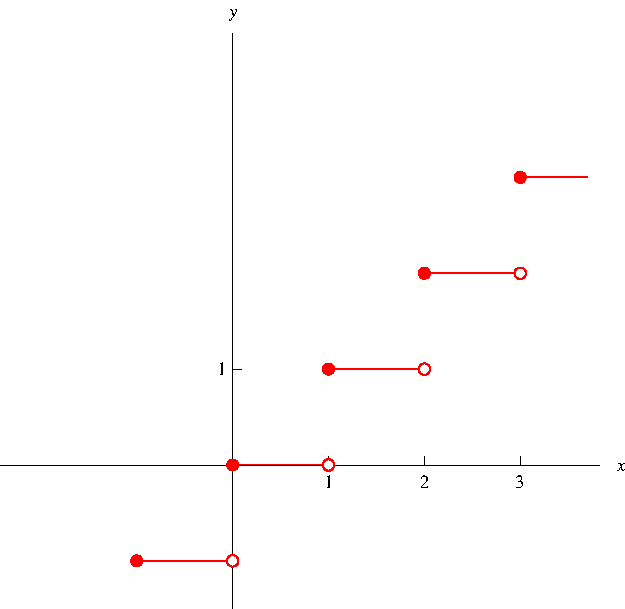
\includegraphics[height=4.5cm]{continuity/pictures/02-05-ex2d.pdf}%

\column{.75\textwidth}
\uncover<2->{%
\[
\begin{array}{@{}r@{~}c@{~}l@{}}
\alertNoH{ 2-3}{\lfloor 4 \rfloor}& \alertNoH{ 2-3}{=}& \fcAnswer{3}{4}\\
\alertNoH{ 4-5}{\lfloor 4.8 \rfloor }&\alertNoH{ 4-5}{=}& \fcAnswer{5}{4}\\
\alertNoH{ 6-7}{\lfloor 1.5\rfloor}&\alertNoH{ 6-7}{=}& \fcAnswer{7}{\lfloor1+0.5\rfloor = 1}\\~\\
\alertNoH{ 8-9,15}{\displaystyle \left\lfloor 1+\frac{1}{2} \right\rfloor}&\alertNoH{8-9,15}{ =}& \fcAnswer{9}{ \alertNoH{15}{1} }\\~\\
\alertNoH{ 10-11}{\displaystyle\left\lfloor \frac{\alertNoH{12}{3} }{2} \right\rfloor} &\alertNoH{10-11}{=}& \displaystyle \fcAnswer{11}{ \left\lfloor\alertNoH{13}{\frac{  \alertNoH{12}{2+1}}{2}} \right\rfloor =
\left \lfloor \alertNoH{13}{ \alertNoH{14}{ \frac{2}{2}} +\frac{1}{2}}\right\rfloor = \alertNoH{15}{ \left\lfloor \alertNoH{ 14}{1}+ \frac{1}{2} \right\rfloor = 1}
}\\~\\
\alertNoH{ 16,17}{\lfloor \pi \rfloor} & \alertNoH{16,17 }{ =}& \fcAnswer{17}{\lfloor 3.1415\dots\rfloor= 3}\\
\end{array}
\]
}
\end{columns}
\end{frame}
% end module greatest-integer-function
